\begin{frame}
  \frametitle{Authentification et contrôle d'accès}
  \begin{block}{\textbf{ Présentation }}
  \begin{itemize}
  \item 
  \item 
  \end{itemize}
  \end{block}
\end{frame}

\begin{frame}
  \frametitle{Authentification et contrôle d'accès}
  \begin{block}{\textbf{Pourquoi un annuaire ? }}
  \begin{itemize}
  \item Plus consulté que mis à jour
  \item Structure hierachique 
  \end{itemize} 
  \end{block}
\end{frame}

\begin{frame}
  \frametitle{Authentification et contrôle d'accès}
  \begin{block}{\textbf{Pourquoi LDAP ? }}
  \begin{itemize}
  \item Protocole réseau léger
  \item Recherche simple et critérisée
  \item Organisation des résultats
  \item Mécanisme de référencement
  \item Authentification et contrôle d'accès
  \item Haute disponibilité via réplication
  \end{itemize}
  \end{block}
\end{frame}

  \frametitle{Authentification et contrôle d'accès}
  \begin{figure}[htbp]
	  \centering
	  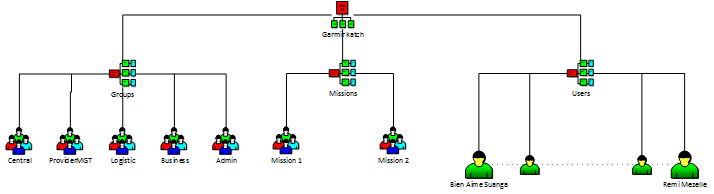
\includegraphics[scale=0.6]{Images/SchemaLDAP.png}
	  \caption{Structure de l'annuaire}
	  \label{SchemaLDAP}
  \end{figure}
 
  \begin{figure}[htbp]
	\centering
	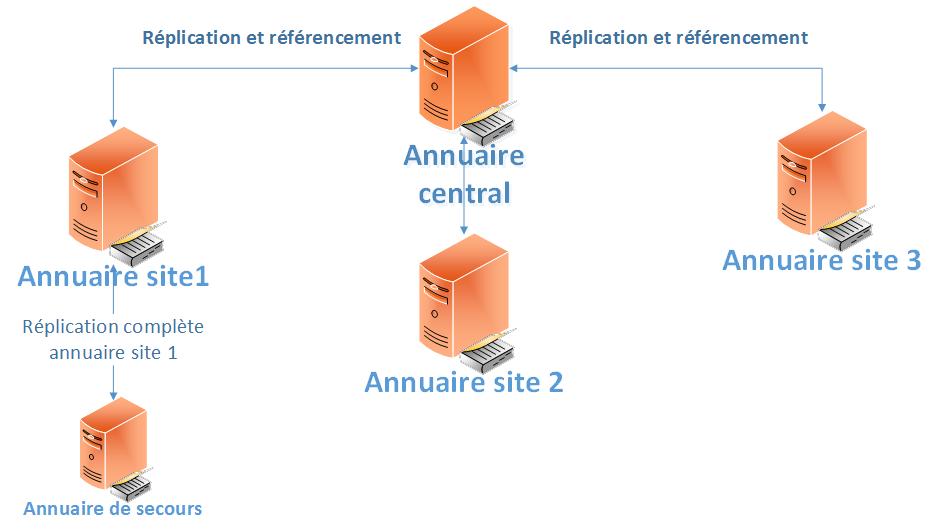
\includegraphics[scale=0.4]{Images/SchemaGlobal.png}
	\caption{Architecture globale}
	\label{SchemaGlobal}
\end{figure}

\begin{figure}[htbp]
	\centering
	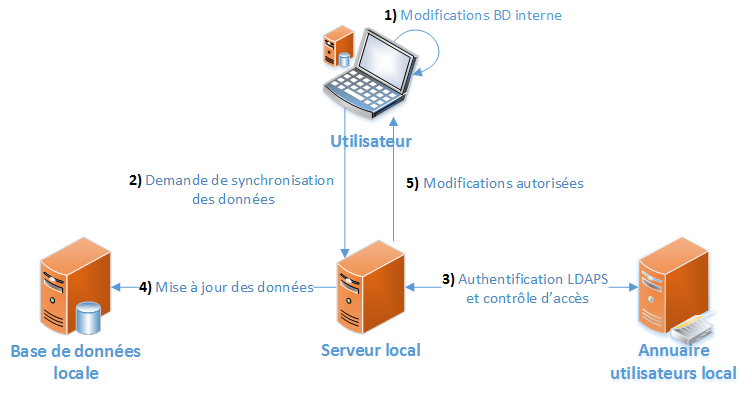
\includegraphics[scale=0.6]{Images/SchemaAuthentification.png}
	\caption{Authentification pour la synchronisation}
	\label{SchemaAuthentification}
\end{figure}

\begin{frame}
  \frametitle{Authentification et contrôle d'accès}
  \begin{block}{\textbf{Droits utilisateurs}}
  \begin{itemize}
  \item Droits pour chaque utilisateur
  \item Droits pour chaque groupe
  \item Autorisations et/ou refus
  \end{itemize}
  \end{block}
\end{frame}

\begin{frame}
  \frametitle{Authentification et contrôle d'accès}
  \begin{block}{\textbf{Contrôle d'accès}}
  \begin{itemize}
  \item Gestion des conflits 
  \item 
  \end{itemize}
  \end{block}
\end{frame}